% Copyright (C) 2009 Thomas L. Kula
% All Rights Reserved
%
% See the file LICENSE for license terms.
\documentclass[12pt]{article}
\usepackage{graphicx}
\usepackage{rotating}
\usepackage{fix-cm}
\setlength{\paperwidth}{5.5in}
\setlength{\paperheight}{8.5in}
\setlength{\textheight}{7.45in}
\setlength{\topmargin}{-1.0in}
\setlength{\oddsidemargin}{-0.5in}
\setlength{\evensidemargin}{-0.5in}
\setlength{\textwidth}{4.0in}
\setlength{\parindent}{0in}
\setlength{\parskip}{3mm}
\usepackage[print]{booklet} \nofiles
\source{\magstep0}{5.5in}{8.5in}
\target{\magstep0}{11in}{8.5in}
\setpdftargetpages
\pagestyle{empty}
\begin{document}


\begin{center}
{\fontsize{36}{48}\selectfont \textsc{Haiku a Day }}
\end{center}

\vspace*{3.5cm}

{\fontsize{26}{52}\selectfont 
An oracle tells 
	 
In blue words, what to do to 
	 
Use the laundromat

}

\vspace*{5.0cm}
\begin{center}
{\large{Issue 53: November 2009}} \\[5mm]
{\fontsize{8}{8}\selectfont  \textsc{ St. Joshua Norton Press }} \\[1mm]
{\fontsize{6}{6}\selectfont Mathom House in Midtown \textbar The People's Republic of Ames }
\end{center}


\newpage

I've realized that in a couple weeks it will be 2010, and I'm
going to have to spend a lot of time re-training my fingers 
from not just putting in a ``00'' without thinking in the
middle of the year. I think I'm going to be typing 20010
a lot....

--- Thomas

http://kula.tproa.net/had/ \\
kula@tproa.net

Download this and previous HADs at the website, so you can
print out your own (DIY, yeah!) or if you want me to send
you one, send me your address, and maybe a stamp if you
are feeling nice. Or send me something you've made ---
trades always appreciated, postcards are nice too.

\vspace*{2cm}

1 November 2009

Weird wireless thing \\
Why do you only half work? \\
What a piece of junk

2 November 2009

Drain running slowly \\
Oh how I am hating you \\
Go faster, dammit

\newpage

3 November 2009

When bits, gathering \\
Coalesce into order \\
Data is produced

4 November 2009

Forgetting to run \\
tune2fs -c  \\
Causes long boot times

5 November 2009

Work today gave me \\
A productivity glow \\
Now I want a nap

6 November 2009

Night in Ann Arbor \\
No one knows how to drive here \\
I'm shaking my fist

7 November 2009

A chill in the air \\
And yet a pot of hot tea \\
Keeps the cold away

8 November 2009

Down into the drome \\
There is shootoff confusion \\
Damn hockey people

9 November 2009

What zine should I read? \\
The pile grows ever large \\
Making a hard choice

\newpage

10 November 2009

Friend Insomnia \\
You got me up too early \\
My head is splitting

11 November 2009

Bored and twisting twine \\
I find I've made a bracelet \\
Close, but not knitting

12 November 2009

The bricks, holding cold \\
Make a chilly atmosphere \\
Ready for sweaters

13 November 2009

Seeking to balance \\
The time spent on many paths \\
Tread lightly, but tread

14 November 2009

Jacket November \\
Leaves me wondering if it \\
Will ever get cold

15 November 2009 

As the sky darkens \\
We do not slow down, we move \\
Where there is bright light

16 November 2009

Walking out at night \\
A quiet city, clear skies \\
And I'm filled with life

\newpage

17 November 2009

The sky slides, tilting \\
Stars becoming a jumble \\
Before they go out

18 November 2009

Speech becoming bits \\
Becoming words on paper \\
An interview done

19 November 2009

The mad rush begins \\
When from vapor words align \\
Fixed eternally

20 November 2009

In the night a bump \\
My toe and the bookcase meet \\
It is not happy

21 November 2009

Start with simple things \\
Complexity will find you \\
Even if you hide

22 November 2009

As I type, grimace \\
Frozen peas ersatz first aid \\
Bring little relief

23 November 2009

And why should I sleep? \\
With every move my thumb screams \\
Oh just chop it off!

\newpage

24 November 2009

Dreaming monopoles \\
Stuck together forever \\
Can they ever be?

25 November 2009

Gimpy hand dishes \\
Should have been done days ago \\
Will I ever learn?

26 November 2009

The gluttony done \\
Lord of the Rings all day long \\
With some random naps

27 November 2009

My usual mix \\
I should be more productive \\
Manage at least some

28 November 2009

Once loud, now murmur \\
Voices ringing out proud, strong \\
Now grow quiet, soft

29 November 2009

In a flash, dark pales \\
And trapped for eternity \\
Light in its fair dance

30 November 2009

The splint is removed \\
Nothing broken, still tender \\
Sad bruises don't scar


\newpage

\begin{center}
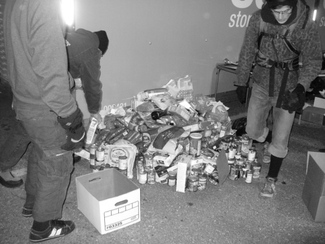
\includegraphics{cranksgiving.jpg} \\[1cm]
What 800 pounds of food looks like \\
Cranksgiving 2009 \\
{\tt http://kula.tproa.net/photos/2009/cranksgiving-2009/ }
\end{center}

\newpage

\thispagestyle{empty}
\vspace*{14cm}
\begin{sideways}
\Large{Thomas L. Kula}
\end{sideways}
\begin{sideways}
\Large{PO Box 980461}
\end{sideways}
\begin{sideways}
\Large{Ypsilanti MI 48198}
\end{sideways}


\end{document}


